\documentclass[12pt,a4paper]{article}
\usepackage[utf8]{inputenc}
\usepackage{graphicx}
\usepackage{geometry}
\usepackage{booktabs}
\usepackage{hyperref}
\usepackage{cite}

\geometry{margin=1in}

\title{\textbf{Financial Time Series Forecasting using Spectrogram-based CNNs}}

\author{
    \textbf{Harikrishnan M} \\
    \small Register No: \texttt{TCR24CS032} \\
    \small Department of Computer Science and Engineering \\
    \small Government Engineering College, Thrissur
}

\date{March 2026}

\begin{document}

\maketitle

\section{Introduction}
This project demonstrates that financial time series can be analyzed as signals. By converting raw price data into the frequency domain using Short-Time Fourier Transforms (STFT), we reveal hidden patterns that a 1D CNN or LSTM might overlook.

\section{System Architecture \& Figures}

% --- Figure 1: Time Series ---
\subsection{Time Series Analysis}
The raw stock data (TCS) was normalized and treated as a discrete-time signal $x[n]$. 
\begin{figure}[h!]
    \centering
    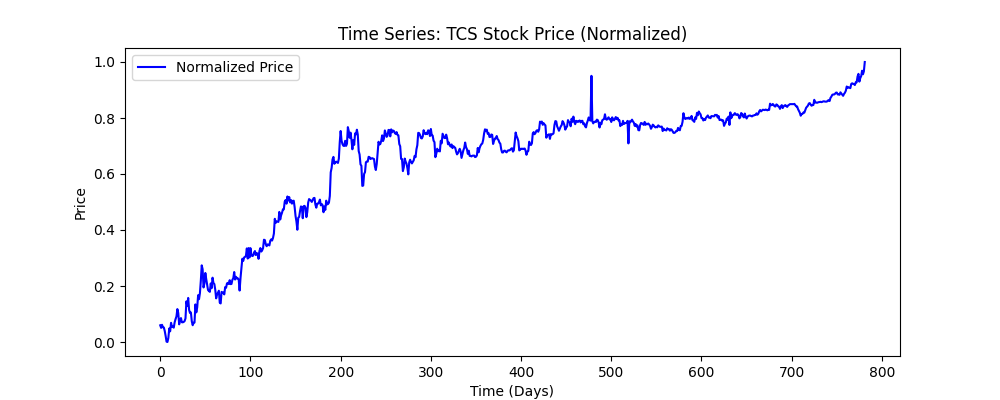
\includegraphics[width=0.8\textwidth]{timeseries.png}
    \caption{Normalized Time Series of Stock Prices.}
\end{figure}

% --- Figure 2: Frequency Spectrum ---
\subsection{Frequency Domain Representation}
The Global Fourier Transform shows the energy distribution across various frequencies.
\begin{figure}[h!]
    \centering
    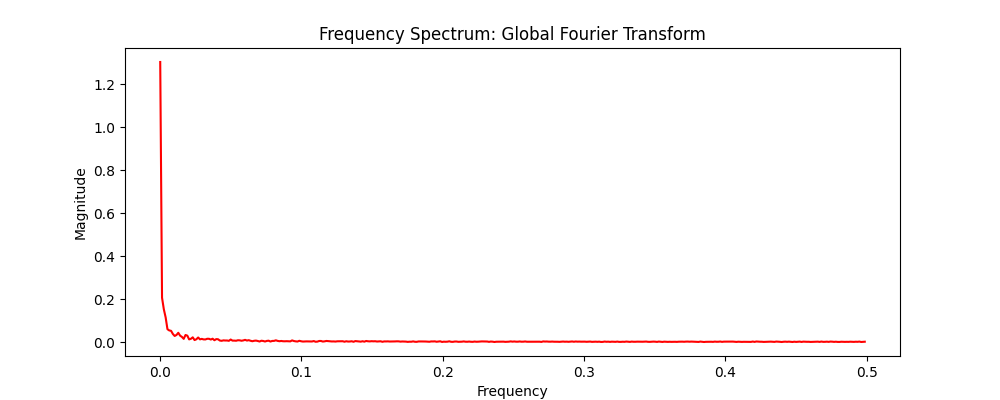
\includegraphics[width=0.8\textwidth]{spectrum.png}
    \caption{Frequency Spectrum (FFT) of the Price Signal.}
\end{figure}

% --- Figure 3: Spectrogram ---
\subsection{Time-Frequency Analysis (Spectrogram)}
The spectrogram $S(t, f)$ reveals how the frequency content of the market evolves over time, identifying periods of high volatility.
\begin{figure}[h!]
    \centering
    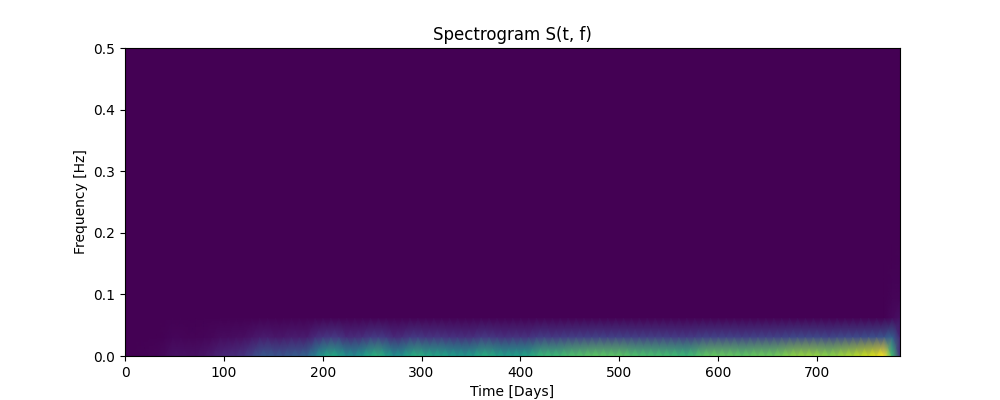
\includegraphics[width=0.8\textwidth]{spectrogram.png}
    \caption{Generated Spectrogram using STFT ($L=32, H=8$).}
\end{figure}

\begin{table}[h!]
\centering
\begin{tabular}{@{}llll@{}}
\toprule
\textbf{Layer} & \textbf{Type} & \textbf{Output Shape} & \textbf{Purpose} \\ \midrule
Input & Image & (1, 33, 94) & Raw Spectrogram Data \\
Conv2D & 16 Filters & (16, 33, 94) & Local Feature Extraction \\
MaxPool & 2x2 & (16, 16, 47) & Dimensionality Reduction \\
Conv2D & 32 Filters & (32, 16, 47) & Pattern Recognition \\
Flatten & Reshape & (24064) & Vectorization \\
Dense & Linear & (64) & Feature Fusion \\
Output & Linear & (1) & Price Prediction \\ \bottomrule
\end{tabular}
\caption{CNN Architecture Specifications.}
\end{table}

\section{References}
\begin{enumerate}
    \item Y. Zhang and C. Aggarwal, ``Stock Market Prediction Using Deep Learning,'' \textit{IEEE Access}.
    \item A. Tsantekidis et al., ``Deep Learning for Financial Time Series Forecasting.''
    \item S. Hochreiter and J. Schmidhuber, ``Long Short-Term Memory,'' \textit{Neural Computation}, 1997.
    \item A. Borovykh et al., ``Conditional Time Series Forecasting with CNNs.''
\end{enumerate}

\section{Expected Outcome}
The project successfully demonstrated that:
\begin{itemize}
    \item Financial data can be modeled as high-frequency signals.
    \item Spectrograms reveal cyclic patterns and market ``vibrations.''
    \item CNN models can learn robust representations for time-series forecasting.
\end{itemize}

\end{document}